\documentclass[11pt]{article}
\usepackage[final]{acl}

\usepackage{times}
\usepackage{latexsym}
\usepackage[T1]{fontenc}
\usepackage[utf8]{inputenc}
\usepackage{microtype}
\usepackage{inconsolata}
\usepackage{graphicx}
\usepackage{booktabs}
\usepackage{multirow}
\usepackage{tabularx}
\usepackage{array}
\usepackage{threeparttable}
\usepackage{siunitx}
\usepackage{amsmath,amssymb}
\usepackage{enumitem}
\usepackage{xspace}
\usepackage[most]{tcolorbox}
\usepackage{subcaption}
\usepackage{hyperref}

\pdfoutput=1
\setlength\titlebox{5.3cm}
\setlength{\tabcolsep}{4.5pt}
\renewcommand{\arraystretch}{1.12}
\setlength{\textfloatsep}{12pt plus 2pt minus 3pt}
\setlength{\floatsep}{10pt plus 2pt minus 2pt}
\setlength{\abovecaptionskip}{5pt}
\setlength{\belowcaptionskip}{0pt}
\urlstyle{same}

\definecolor{accent}{HTML}{0D5C63}
\definecolor{accent2}{HTML}{A63D40}
\definecolor{lightgraybg}{HTML}{F5F7F8}
\definecolor{softgray}{HTML}{70757A}

\newcommand{\paperTitle}{When Accuracy Hides Path Dependence: Criterion Fidelity in LLM Judges}
\newcommand{\qwen}{Qwen2.5-14B-Instruct\xspace}
\newcommand{\llama}{Llama-3.1-8B-Instruct\xspace}
\newcommand{\qwenS}{Qwen-14B\xspace}
\newcommand{\llamaS}{Llama-8B\xspace}
\newcommand{\qakey}{QA-Key\xspace}
\newcommand{\biorubric}{BioRubric\xspace}
\newcommand{\baseacc}{\textsc{BaseAcc}\xspace}
\newcommand{\gcf}{\textsc{GCF}\xspace}
\newcommand{\sens}{\textsc{Sens@BC}\xspace}
\newcommand{\invbc}{\textsc{Inv@BC}\xspace}
\newcommand{\orderdis}{\textsc{OrderDisagreement}\xspace}
\newcommand{\gap}{\textsc{Gap}\xspace}
\newcommand{\stdprompt}{standard\xspace}
\newcommand{\strictprompt}{strict criterion-emphasis\xspace}

\sisetup{
  round-mode=places,
  round-precision=3,
  group-digits=false,
  detect-weight=true,
  detect-family=true,
  table-number-alignment=center
}

\title{\paperTitle}
\author{Ali Uyar\\Independent Researcher}

\begin{document}
\maketitle

\begin{abstract}
Large language model judges are commonly validated by ordinary task accuracy or judge--reference agreement, implicitly assuming that a judge that looks accurate is following the provided criterion. We argue that this is incomplete: in criterion-conditioned evaluation, a valid judge should change when the criterion meaning changes and remain stable when wording changes but meaning does not. We formalize this property as \emph{criterion fidelity} and measure it with \emph{criterion families}---matched groups of base, paraphrase, and counterfactual variants evaluated with mirrored-order continuation scoring. Across two controlled task families---\qakey, a high-margin keyed-answer setting, and \biorubric, a low-margin rubric-conditioned pairwise setting where both candidates are factually true---ordinary quality and criterion fidelity dissociate. Under standard prompting, \qakey gaps are small but real, while \biorubric gaps are large: for \qwen, \baseacc$=0.783$ but \gcf$=0.498$; for \llama, \baseacc$=0.727$ but \gcf$=0.217$. Strict criterion-emphasis prompting is not a reliable remedy: it removes the gap on \qakey/\qwen, narrows it on \biorubric/\qwen, and worsens both quality and order instability on \biorubric/\llama. Failure analysis shows that underreaction to criterion changes dominates paraphrase instability, but the largest rubric-based failures are often mediated by presentation-sensitive path dependence rather than by a clean majority of direct semantic criterion refusal. On the most pathological slice, \llama evaluated with the strict prompt becomes nearly a pure first-position chooser on \biorubric while remaining almost balanced over underlying candidate identity. These results position criterion fidelity as a distinct validity axis for LLM judges and show that criterion-conditioned instability, not just answer-level inaccuracy, should be part of judge evaluation.
\end{abstract}

\section{Introduction}
Large language models are increasingly used as judges: to score candidate outputs, compare systems, filter synthetic data, and stand in for more expensive human evaluation \citep{chiang2023can,zheng2023judging}. In practice, these uses are often validated with ordinary accuracy, agreement, or correlation. That standard is useful, but it quietly assumes something stronger: if a judge gets the base case right, then it must be implementing the provided criterion.

This assumption is testable and incomplete. A judge can be \emph{right for the wrong reason}. In criterion-conditioned evaluation, the input, candidate outputs, and rubric or reference are all part of the object being judged. A model that selects the right winner on the base item but fails to change when the criterion changes, or flips when the criterion wording changes but its meaning does not, is not faithfully implementing the criterion even if its base accuracy looks respectable.

We study this property as \emph{criterion fidelity}. Rather than flattening evaluation into independent rows, we group matched items into \emph{criterion families}: a base variant, two meaning-preserving paraphrases, and a counterfactual criterion that should flip the winner. This gives a direct test of whether a judge's decision is actually controlled by the criterion. We evaluate two controlled families. \qakey provides a high-margin keyed-answer setting close to reference-based question answering. \biorubric provides a harder rubric-conditioned pairwise setting in which both candidates are factually true and only the rubric weights determine the winner.

The resulting picture is sharper---and more interesting---than the narrower ``judges choose beliefs over criteria'' story. We find that ordinary judge quality and criterion fidelity dissociate on both task families, with especially large gaps on \biorubric. We also find that these failures are not dominated by a clean majority of direct semantic criterion refusal. Instead, the largest rubric-based failures are often mediated by presentation-sensitive path dependence: the decision depends on candidate serialization even after mirrored-order aggregation, and stronger criterion-emphasis prompting does not reliably fix this pathology. On the most extreme slice, \llama under the strict prompt is almost a pure first-position chooser on \biorubric.

Our contribution is therefore a validity paper, not a new judge benchmark. We make four claims supported by the completed evidence. First, ordinary judge quality is not the same as criterion fidelity. Second, the gap is not only a knowledge-conflict artifact: it appears in a non-QA family where both candidates are true. Third, failures decompose into underreaction and overreaction, with underreaction dominant on the meaningful slices. Fourth, strict criterion-emphasis prompting is an unreliable baseline rather than a solution. A narrower mechanism claim---that the largest failures are mostly direct semantic refusal to follow the criterion---is only partially supported and is treated as such.

\section{Criterion Fidelity as a Family-Level Validity Property}
\label{sec:framework}

\begin{figure*}[t]
  \centering
  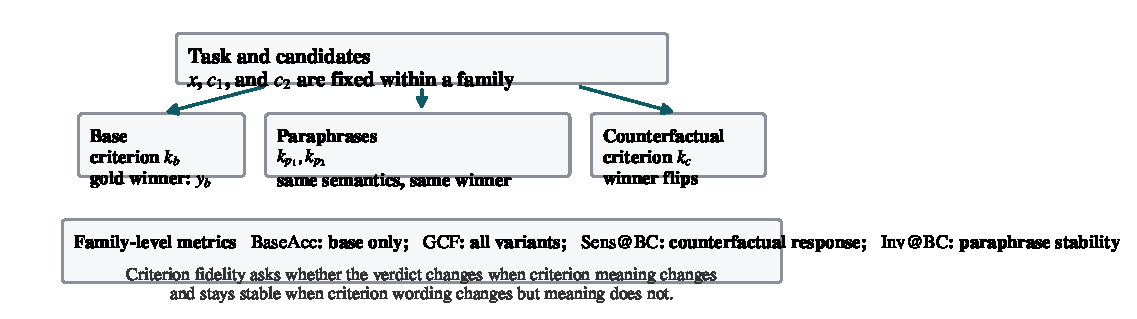
\includegraphics[width=0.92\textwidth]{figures/criterion_family_schematic.pdf}
  \caption{Criterion families keep the task and candidates fixed while varying only the criterion. A judge with high criterion fidelity should change when the counterfactual criterion changes the gold winner and remain stable when paraphrases preserve criterion meaning.}
  \label{fig:family-schematic}
\end{figure*}

A criterion family $f$ contains a fixed task input $x_f$, two underlying candidates $c_{f,1}$ and $c_{f,2}$, and four logical variants $v \in \{b,p_1,p_2,c\}$: one base criterion, two paraphrases that preserve criterion semantics, and one counterfactual criterion that flips the gold winner. The family is the evaluation unit.

For each logical variant we evaluate both candidate orders, $o\in\{AB,BA\}$. Let $\pi_{f,v,o}$ be the rendered chat prefix that ends immediately before the answer label, and let $\lambda_o(c)\in\{A,B\}$ be the displayed label of underlying candidate $c$ under order $o$. We score literal continuations ``A'' and ``B'' by continuation log-probability from the identical rendered prefix and then remap both orders back to underlying candidate IDs:
\begin{equation}
S_{f,v}(c) = \frac{1}{2}\sum_{o\in\{AB,BA\}} \log p_\theta\!\left(\lambda_o(c)\mid \pi_{f,v,o}\right).
\end{equation}
We predict the higher-scoring underlying candidate unless $|S_{f,v}(c_{f,1}) - S_{f,v}(c_{f,2})| \le \varepsilon$ with $\varepsilon = 10^{-6}$, in which case we record a tie. Ties are logged and counted incorrect for the binary headline metrics.

This setup separates three distinct questions. Ordinary quality asks whether the base item is correct. Criterion sensitivity asks whether the judge responds correctly when the criterion semantics change. Criterion invariance asks whether the judge remains correct when the criterion wording changes without semantic change. We report four family-level headline metrics:
{\small
\begin{align}
\baseacc &= \frac{1}{|\mathcal{F}|}\sum_f \mathbf{1}[\hat y_{f,b}=y_{f,b}],\\
\gcf &= \frac{1}{|\mathcal{F}|}\sum_f \mathbf{1}[\forall v\in\{b,p_1,p_2,c\}:\hat y_{f,v}=y_{f,v}],\\
\sens &= \frac{\sum_f \mathbf{1}[\hat y_{f,b}=y_{f,b}\wedge \hat y_{f,c}=y_{f,c}]}{\sum_f \mathbf{1}[\hat y_{f,b}=y_{f,b}]},\\
\invbc &= \frac{\sum_f \mathbf{1}[\hat y_{f,b}=y_{f,b} \wedge \hat y_{f,p_1}=y_{f,p_1}]}{\sum_f \mathbf{1}[\hat y_{f,b}=y_{f,b}]} \\
&\qquad \times \mathbf{1}[\hat y_{f,p_2}=y_{f,p_2}].
\end{align}
}
We refer to $1-\sens$ as \emph{underreaction} and $1-\invbc$ as \emph{overreaction}. As supporting diagnostics we also report \orderdis, the fraction of logical variants whose $AB$ and $BA$ order-specific decisions disagree before aggregation, and the tie rate after mirrored-order aggregation.

Two aspects of the framework matter for interpretation. First, the family-level metrics are intentionally harsher than row-wise accuracy: a family fails \gcf if \emph{any} of its four logical variants fails. Second, mirrored-order evaluation does not create path dependence; it reveals it. If a judge behaves differently across candidate serializations, criterion-conditioned evaluation is already unstable.

\section{Controlled Task Families}
\label{sec:tasks}

\begin{table}[t]
  \centering
  \small
  \begin{threeparttable}
  \caption{Controlled task families. Both families use frozen splits of 2000/400/600 criterion families for train/dev/test.}
  \label{tab:datasets}
  \begin{tabularx}{\columnwidth}{@{}l>{\raggedright\arraybackslash}Xc>{\raggedright\arraybackslash}X@{}}
    \toprule
    Task family & Controlled object & Built families & Key caveat \\
    \midrule
    \qakey & Keyed-answer preference under controlled answer-key swaps over six Wikidata relations spanning place, date, capital, and currency. & 6,168 & High-margin setting: one candidate matches the key and the other does not. Useful anchor, but still close to reference-conditioned QA. \\
    \addlinespace[2pt]
    \biorubric & Two-sentence biographies built from Wikidata truthy statements. Both candidates are factual, share one fact, and differ on one rubric-weighted fact from the same slot. & 4,385 & Low-margin comparative setting: the criterion must determine which true candidate is preferred. This is the decisive non-QA family. \\
    \bottomrule
  \end{tabularx}
  \end{threeparttable}
\end{table}

\qakey and \biorubric are designed to isolate criterion dependence under different margins and different failure temptations.

\paragraph{QA-Key.}
\qakey is a controlled keyed-answer family built from six Wikidata-backed relations: place of birth, place of death, date of birth, date of death, capital, and currency. Each family fixes a question and two answer candidates. The base criterion is an official answer key; the counterfactual criterion swaps in a donor answer from the same relation and coarse answer type; the paraphrases preserve answer-key semantics. This family gives a clean high-margin test close to reference-conditioned QA, and therefore remains the most natural place to observe direct semantic criterion failures of the kind highlighted by \citet{lee2026judging}.

\paragraph{BioRubric.}
\biorubric removes knowledge-conflict as the dominant explanation. Each family describes a human entity using two deterministic two-sentence biographies built from Wikidata truthy statements. The biographies share one occupation fact and differ on one additional fact drawn from the same slot type (notable work, award, or field). The criterion is an explicit weighted rubric: in the base variant one distinguishing fact receives higher weight; in the counterfactual variant the other distinguishing fact receives higher weight; paraphrases preserve the rubric semantics. Both candidates are factual. The only thing that should change the winner is the criterion.

The final frozen source contains 6,256 raw \qakey rows, which become 6,174 canonical rows and 6,168 valid built families before split truncation. For \biorubric, 55,854 truthy fact rows over 5,081 entities become 4,385 valid built families before split truncation. We freeze both families to train/dev/test sizes of 2000/400/600 and keep the processed datasets immutable for the headline results.

\section{Ordinary Quality Hides Criterion-Fidelity Failure}
\label{sec:main-results}

\begin{table*}[t]
  \centering
  \small
  \begin{threeparttable}
  \caption{Standard-prompt headline results on the frozen test sets. \gap $= \baseacc - \gcf$. All confidence intervals are 95\% family bootstrap intervals.}
  \label{tab:main-results}
  \begin{tabular}{@{}llccccccc@{}}
    \toprule
    Task & Model & \baseacc & \gcf & \gap [95\% CI] & \sens & \invbc & Order dis. & Tie \\
    \midrule
    \qakey & \qwenS & 1.000 & 0.983 & 0.017 [0.007, 0.027] & 0.985 & 0.998 & 0.007 & 0.0004 \\
    \qakey & \llamaS & 1.000 & 0.972 & 0.028 [0.015, 0.042] & 0.972 & 1.000 & 0.180 & 0.0000 \\
    \midrule
    \biorubric & \qwenS & 0.783 & 0.498 & 0.285 [0.250, 0.322] & 0.740 & 0.896 & 0.292 & 0.0029 \\
    \biorubric & \llamaS & 0.727 & 0.217 & 0.510 [0.468, 0.550] & 0.429 & 0.775 & 0.944 & 0.0354 \\
    \bottomrule
  \end{tabular}
  \end{threeparttable}
\end{table*}

\begin{figure}[t]
  \centering
  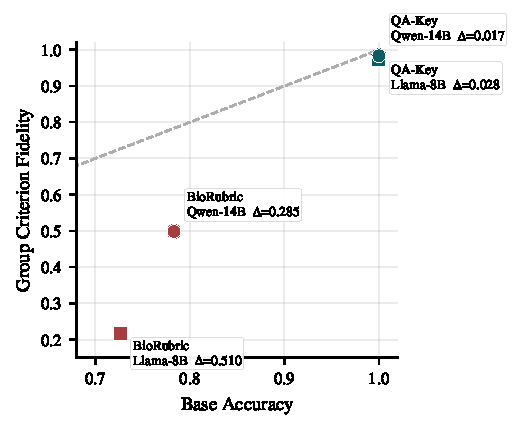
\includegraphics[width=0.98\columnwidth]{figures/baseacc_vs_gcf_refined.pdf}
  \caption{\baseacc versus \gcf under standard prompting. The QA slices cluster near the top-right with small but nonzero gaps. The decisive result is \biorubric, where ordinary quality looks much better than family-level criterion fidelity.}
  \label{fig:baseacc-vs-gcf}
\end{figure}

Table~\ref{tab:main-results} and Figure~\ref{fig:baseacc-vs-gcf} establish the paper's central empirical result. Ordinary judge quality and criterion fidelity are not the same object. On \qakey, the dissociation is modest but statistically real under standard prompting for both models. On \biorubric, the dissociation is large and decisive: \qwen loses 0.285 points from \baseacc to \gcf, and \llama loses 0.510.

This immediately gives two conclusions. First, criterion fidelity is distinct from ordinary judge quality. Second, the gap is not only a knowledge-conflict artifact. \biorubric is the crucial family here: both candidates are true, and the gold winner changes only because the rubric changes. The BioRubric results therefore show a criterion-conditioned validity failure in a setting where the judge cannot lean on factual correctness alone.

The decomposition into sensitivity and invariance clarifies the structure of the gap. On the large-gap slices, \sens is systematically below \invbc. For \qwen on \biorubric under the standard prompt, \sens is 0.740 while \invbc is 0.896; for \llama the gap is even larger, 0.429 versus 0.775. The dominant failure is therefore \emph{underreaction}: the judge fails more often when criterion semantics change than when criterion wording changes but its meaning does not.

This does not mean that paraphrase instability is absent. Rather, it means that the main failure is not ordinary phrasing brittleness. The judges often fail to let the criterion change control the verdict strongly enough. That is already visible in \qakey, but it becomes unmistakable in \biorubric.

\section{Strict Criterion-Emphasis Prompting Is Not a Reliable Remedy}
\label{sec:strict}

\begin{figure*}[t]
  \centering
  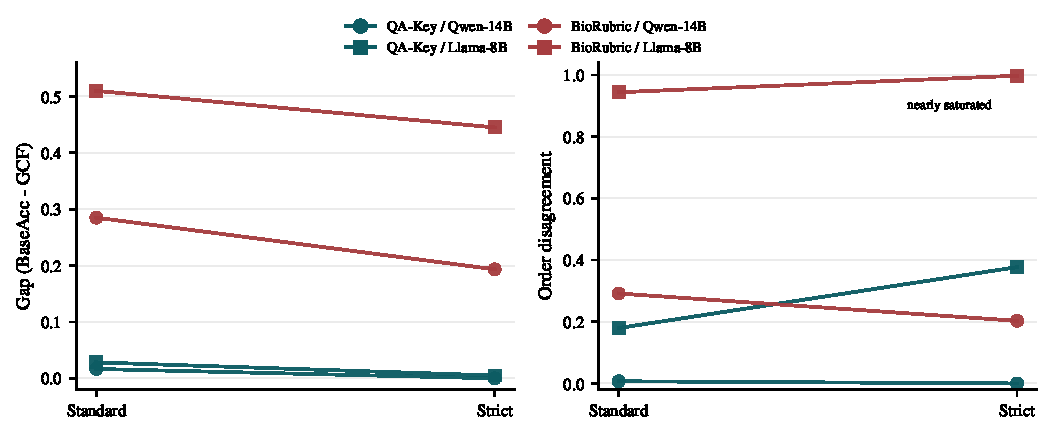
\includegraphics[width=0.94\textwidth]{figures/strict_gap_order_refined.pdf}
  \caption{Effect of the strict criterion-emphasis prompt relative to the standard prompt. Left: criterion-fidelity gap. Right: order disagreement. Strict prompting helps some slices, but it is not a reliable remedy and can amplify instability.}
  \label{fig:strict-deltas}
\end{figure*}

A natural baseline is to instruct the model more forcefully to follow the criterion exactly. Figure~\ref{fig:strict-deltas} shows why this is not the paper's story.

On \qakey, stricter prompting can remove or nearly remove the gap. For \qwen, the standard-prompt gap of 0.017 collapses to 0.000. For \llama, the gap drops from 0.028 to 0.005. These improvements are real, but they occur in the high-margin keyed-answer family where the criterion signal is already strong.

On \biorubric, the picture is qualitatively different. \qwen improves, but the problem remains: \baseacc rises from 0.783 to 0.863, \gcf from 0.498 to 0.670, and the gap remains a substantial 0.193. \llama is worse. Under the strict prompt, \baseacc falls from 0.727 to 0.577, \gcf falls from 0.217 to 0.132, order disagreement rises from 0.944 to 0.998, and the tie rate more than doubles to 0.0879.

The lesson is not that prompting never matters. It clearly does. The lesson is that stronger criterion-emphasis instructions do not reliably make the criterion control the decision. On some slices they help, on others they leave a large residual gap, and on the most pathological slice they amplify the wrong signal.

\section{Path Dependence in Rubric-Conditioned Evaluation}
\label{sec:path}

\begin{figure*}[t]
  \centering
  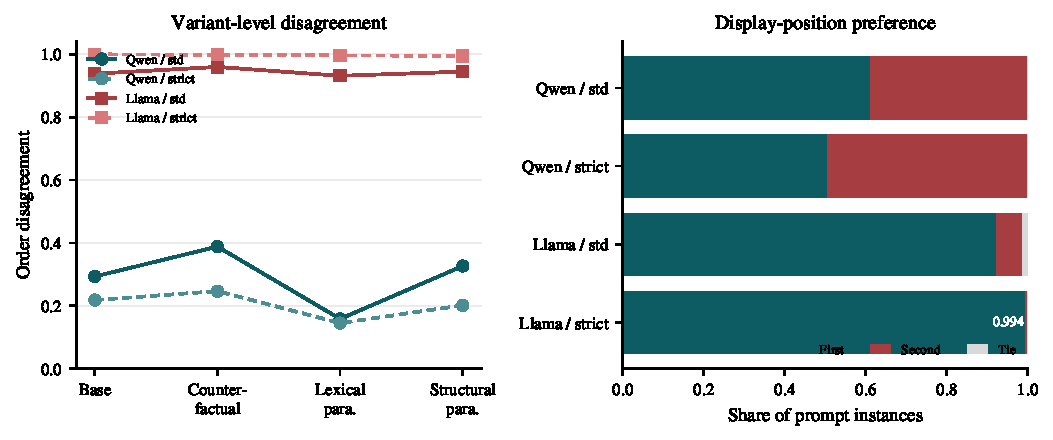
\includegraphics[width=0.95\textwidth]{figures/biorubric_path_dependence.pdf}
  \caption{Path-dependence diagnostics on \biorubric. Left: variant-level order disagreement is highest on the counterfactual variants for \qwen and is nearly saturated across all variants for \llama. Right: display-position preference reveals the extreme strict-prompt \llama pathology: nearly every prompt instance chooses the first-presented candidate even though the underlying candidate identity remains nearly balanced.}
  \label{fig:path-dependence}
\end{figure*}

The key question after the main results is what kind of failure produces the large \biorubric gaps. The audits and diagnostics point to a clear answer: on the largest-gap slices, criterion-fidelity failure is often mediated by presentation-sensitive path dependence.

Manual audits make the pattern concrete. On \biorubric under standard prompting, \texttt{order\_effect} accounts for 34/50 audited failures for \qwen and 36/50 for \llama. Under strict prompting, the same label still dominates (32/50 for \qwen and 36/50 for \llama), and \llama adds 14/50 audited \texttt{model\_tie} cases. Direct semantic criterion failures remain visible---for example, 15/50 audited \qwen standard failures and 17/50 audited \qwen strict failures are labeled \texttt{genuine\_criterion\_failure}---but they are not the majority channel on the largest-gap slices.

This does \emph{not} mean the criterion is irrelevant and only order matters. It means that the observable route by which the criterion fails to control the verdict is often order-sensitive instability. The difference matters. A model can fail criterion-conditioned evaluation because it refuses the criterion semantically, because it is brittle to criterion wording, or because its pairwise decision process is path dependent. The completed evidence says that the last route is a major part of the story in close rubric-based settings.

The diagnostics sharpen this claim. First, order disagreement is highest exactly where criterion sensitivity should matter most. For \qwen on \biorubric under the standard prompt, the counterfactual variant has the highest disagreement rate (0.388). Under the strict prompt it remains the most unstable variant (0.247). Second, restricting to order-stable families does not eliminate the issue on \qwen. The \biorubric gap remains 0.217 on order-stable families under the standard prompt and 0.123 under the strict prompt (Appendix~\ref{fig:appendix-order-stability}). Path dependence therefore explains a large part of the failure, but not all of it.

For \llama, however, path dependence is the main event. Under standard prompting, 599 of 600 \biorubric families are order-unstable. Under strict prompting, \emph{every} test family is order-unstable. The right panel of Figure~\ref{fig:path-dependence} shows what this instability looks like in practice. On \biorubric with the strict prompt, \llama chooses the first-presented candidate 99.44\% of the time, the second-presented candidate only 0.46\% of the time, and yet remains almost perfectly balanced over the underlying candidate identities because mirrored-order evaluation presents each candidate first half the time. This is not random noise. It is a serialization pathology that breaks criterion-conditioned pairwise evaluation.

\begin{tcolorbox}[enhanced, colback=lightgraybg, colframe=black!35, sharp corners, boxrule=0.5pt, left=4pt, right=4pt, top=4pt, bottom=4pt]
\textbf{Representative failure (BioRubric / Llama / standard).} In the family for \emph{Loretta Graziano Breuning}, both biographies are factual and share the same occupation: one says she worked in \emph{happiness}, the other in \emph{management}. The base rubric rewards \emph{happiness} more heavily; the counterfactual rewards \emph{management}. Llama disagrees across candidate orders on all four logical variants and ends up predicting the wrong winner on both the base and counterfactual variants. This is criterion-conditioned invalidity in a non-QA setting, mediated by path dependence rather than by a simple factual conflict.
\end{tcolorbox}

This example also clarifies why the paper remains stronger as a validity paper than as a narrow ``belief override'' paper. Clean direct semantic failures do occur: \qakey provides them, and some \biorubric families do as well. But the largest rubric-based failures are often failures of \emph{stable criterion implementation}. The judge is not simply choosing its own preferred answer over the criterion; it is failing to realize the same criterion-conditioned comparison consistently across equivalent serializations.

\section{Discussion and Limitations}
\label{sec:discussion}

The main lesson is that criterion fidelity is a reusable validity axis for LLM judges. A judge can look accurate on the base item while failing the stronger requirement that it respond correctly to criterion changes and remain stable under criterion-preserving rewordings. In that sense, criterion fidelity is not another accuracy metric. It asks whether the judge is implementing the intended evaluation function.

The paper is also clearest about what it \emph{does not} show. The strongest completed evidence does not support the broad claim that LLM judges mostly ignore criteria in favor of their own beliefs. That narrower mechanism appears in some \qakey cases and in some audited \biorubric failures, but it does not dominate the large-gap rubric slices. The more honest and stronger statement is that ordinary judge quality can hide criterion-conditioned instability, and that in close rubric-conditioned pairwise settings this instability is often presentation-sensitive.

This reframing makes the BioRubric result more interesting, not less. Position bias and serialization effects in LLM judges have been noted before \citep{zheng2023judging,shi2024judging,xu2026pointwise}. Our result is different in two ways. First, the pathology is measured against a criterion-conditioned validity object rather than against generic agreement alone. Second, the pathology appears in a setting where both candidates are true and the criterion should be the decisive signal. In that setting, path dependence is not a nuisance confound on top of the main result. It is one of the main ways criterion fidelity fails.

The strict-prompt results reinforce this point. Extra criterion emphasis helps only when the base decision problem is already high margin, and it can make the low-margin rubric task worse. On \llama/\biorubric, the strict prompt seems to sharpen the wrong comparator: the model becomes more serialization-sensitive and less criterion-faithful at the same time. ``Reminding'' the model to follow the criterion is not equivalent to making the criterion causally control the decision.

Our study has several limits. It uses controlled tasks rather than naturally occurring evaluation pipelines; the models are two open instruct models rather than the full judge ecosystem; and the paper stops short of proposing a mainline mitigation. These are deliberate choices. The goal is not a new benchmark suite or a benchmark-sprawl survey, but a clean validity test. The controlled families let us keep the task and candidates fixed while changing only the criterion, and that is exactly what makes the resulting failures interpretable.

\section{Conclusion}
We introduced criterion fidelity as a family-level validity axis for LLM judges and evaluated it on two controlled task families. Ordinary judge quality and criterion fidelity dissociate even in a high-margin QA setting and diverge sharply in a non-QA rubric-conditioned family. The resulting failures are not captured by ordinary base accuracy and are not reliably repaired by stronger criterion-emphasis prompts. In the hardest rubric-based slices, criterion-fidelity failure is often mediated by order-sensitive path dependence rather than by a clean majority of direct semantic criterion refusal. For judge evaluation, that is the main takeaway: accuracy alone can hide whether a model is actually implementing the criterion.

\begin{thebibliography}{5}
\small

\bibitem[Chiang and Lee(2023)]{chiang2023can}
Cheng-Han Chiang and Hung-yi Lee. 2023.
\newblock Can large language models be an alternative to human evaluations?
\newblock In \emph{Proceedings of the 61st Annual Meeting of the Association for Computational Linguistics}.

\bibitem[Lee et~al.(2026)]{lee2026judging}
Dongryeol Lee, Yerin Hwang, Taegwan Kang, Minwoo Lee, Younhyung Chae, and Kyomin Jung. 2026.
\newblock Judging against the reference: Uncovering knowledge-driven failures in {LLM}-judges on {QA} evaluation.
\newblock \emph{arXiv preprint arXiv:2601.07506}.

\bibitem[Shi et~al.(2024)]{shi2024judging}
Lin Shi, Chiyu Ma, Wenhua Liang, Weicheng Ma, and Soroush Vosoughi. 2024.
\newblock Judging the judges: A systematic study of position bias in {LLM}-as-a-judge.
\newblock \emph{arXiv preprint arXiv:2406.07791}.

\bibitem[Xu et~al.(2026)]{xu2026pointwise}
Yuzheng Xu, Tosho Hirasawa, Tadashi Kozuno, and Yoshitaka Ushiku. 2026.
\newblock Am {I} more pointwise or pairwise? Revealing position bias in rubric-based {LLM}-as-a-judge.
\newblock \emph{arXiv preprint arXiv:2602.02219}.

\bibitem[Zheng et~al.(2023)]{zheng2023judging}
Lianmin Zheng, Wei-Lin Chiang, Ying Sheng, Siyuan Zhuang, Zhanghao Wu, Yonghao Zhuang, Zi Lin, Zhuohan Li, Dacheng Li, Eric P. Xing, Hao Zhang, Joseph E. Gonzalez, and Ion Stoica. 2023.
\newblock Judging {LLM}-as-a-judge with {MT}-Bench and Chatbot Arena.
\newblock \emph{arXiv preprint arXiv:2306.05685}.

\end{thebibliography}

\clearpage
\appendix
\onecolumn

\section{Additional Metrics and Diagnostics}

\begin{center}
  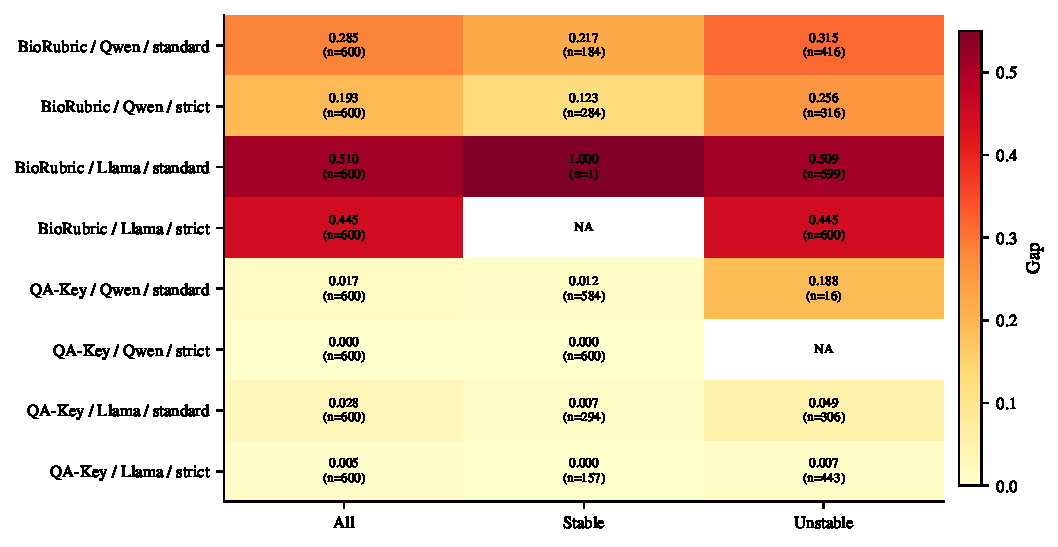
\includegraphics[width=0.82\textwidth]{figures/order_stability_gap_appendix.pdf}
  {\captionsetup{hypcap=false}\captionof{figure}{Gap decomposition by order stability. On \qwen/\biorubric, a substantial residual gap remains even after restricting to order-stable families. On \llama/\biorubric, almost every family is order-unstable, so path dependence dominates the slice.}}
  \label{fig:appendix-order-stability}
\end{center}

\begin{center}
  {\captionsetup{hypcap=false}\captionof{table}{Strict-prompt deltas relative to the standard prompt. Positive values indicate an increase under the strict prompt.}}
  \label{tab:strict-deltas}
  \small
  \begin{tabular}{@{}llcccccc@{}}
    \toprule
    Task & Model & $\Delta$Base & $\Delta$GCF & $\Delta$Gap & $\Delta$Sens & $\Delta$Inv & $\Delta$Order \\
    \midrule
    \qakey & \qwenS & $\phantom{-}0.000$ & $\phantom{-}0.017$ & $-0.017$ & $\phantom{-}0.015$ & $\phantom{-}0.002$ & $-0.007$ \\
    \qakey & \llamaS & $-0.020$ & $\phantom{-}0.003$ & $-0.023$ & $\phantom{-}0.023$ & $\phantom{-}0.000$ & $\phantom{-}0.197$ \\
    \midrule
    \biorubric & \qwenS & $\phantom{-}0.080$ & $\phantom{-}0.172$ & $-0.092$ & $\phantom{-}0.109$ & $\phantom{-}0.031$ & $-0.089$ \\
    \biorubric & \llamaS & $-0.150$ & $-0.085$ & $-0.065$ & $-0.030$ & $-0.099$ & $\phantom{-}0.054$ \\
    \bottomrule
  \end{tabular}
\end{center}

\begin{center}
  {\captionsetup{hypcap=false}\captionof{table}{Failure-audit summary for the principal slices. The audit taxonomy gives \texttt{order\_effect} precedence over \texttt{genuine\_criterion\_failure}; percentages therefore describe the observed failure channel rather than an exhaustive partition of all conceptual criterion failures.}}
  \label{tab:audit-summary}
  \small
  \begin{tabular}{@{}llcccc@{}}
    \toprule
    Slice & $n_{\text{aud}}$ & Genuine criterion failure & Order effect & Model tie & Other \\
    \midrule
    QA-Key / Qwen / standard & 10 & 70\% & 20\% & 10\% & 0\% \\
    QA-Key / Llama / standard & 17 & 24\% & 76\% & 0\% & 0\% \\
    BioRubric / Qwen / standard & 50 & 30\% & 68\% & 2\% & 0\% \\
    BioRubric / Llama / standard & 50 & 6\% & 72\% & 22\% & 0\% \\
    BioRubric / Qwen / strict & 50 & 34\% & 64\% & 2\% & 0\% \\
    BioRubric / Llama / strict & 50 & 0\% & 72\% & 28\% & 0\% \\
    \bottomrule
  \end{tabular}
\end{center}

\begin{center}
  {\captionsetup{hypcap=false}\captionof{table}{Variant-level order disagreement and position preference on the BioRubric slices. The strict-prompt Llama slice is nearly a pure first-position chooser while remaining almost balanced over the underlying candidate identities.}}
  \label{tab:variant-order}
  \small
  \begin{tabular}{@{}llcccccccc@{}}
    \toprule
    Slice & Base & CF & Para 1 & Para 2 & First-pos & Second-pos & Tie & Choose $c_1$ & Choose $c_2$ \\
    \midrule
    BioRubric / Qwen / standard & 0.293 & 0.388 & 0.158 & 0.327 & 0.612 & 0.388 & 0.0002 & 0.632 & 0.368 \\
    BioRubric / Llama / standard & 0.945 & 0.958 & 0.932 & 0.945 & 0.922 & 0.066 & 0.0117 & 0.515 & 0.473 \\
    BioRubric / Qwen / strict & 0.218 & 0.247 & 0.145 & 0.202 & 0.506 & 0.493 & 0.0006 & 0.672 & 0.327 \\
    BioRubric / Llama / strict & 1.000 & 0.998 & 0.997 & 0.995 & 0.994 & 0.0046 & 0.0010 & 0.500 & 0.499 \\
    \bottomrule
  \end{tabular}
\end{center}
\clearpage

\section{Representative Examples}

\paragraph{Clean direct criterion failure (QA-Key / Qwen / standard).}
For the question ``What currency is used in Sao Tome and Principe?'', the candidates are ``The answer is Sao Tome and Principe dobra'' and ``The answer is Eastern Caribbean dollar.'' Under the base criterion, the gold winner is the dobra candidate; under the counterfactual criterion, the gold winner flips to the Eastern Caribbean dollar. Qwen predicts the dobra candidate on all four variants with no order disagreement or ties. This is a clean direct semantic criterion failure.

\paragraph{Strict-prompt serialization pathology (BioRubric / Llama / strict).}
For the Claude Sautet family, both biographies are factual and differ only in the cited work. Under the strict prompt, all four logical variants are order-disagreeing, the base variant collapses to a tie, and the slice-level statistics show a first-position selection rate of 0.994 while the underlying candidate identity remains nearly balanced. This is the clearest failure case for the claim that stronger criterion emphasis is not equivalent to stronger criterion control.

\end{document}
